%describe the tasks to be completed that will satisfy the given objective
\section{Activity}
\noindent
For this lab, you will be developing two classes: a CameraActivity and an EditActivity class. The camera capabilities on the Android phone will be utilized. You will be required to code each of these objects in a way that they can interact with each other to accomplish the task of capturing a picture and editing that picture.

\noindent
The CameraActivity class should be able to take a picture with the camera, and then send it to the EditActivity class to be maniplulated by the user. Below is a screenshot of the app you will be creating.

\begin{center}
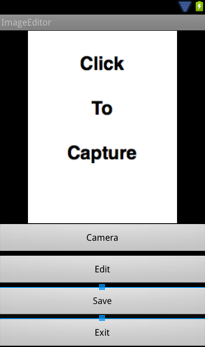
\includegraphics[scale=0.4]{screenshot.png} 
\end{center}
\subsection{Implementation}
This section will guide you through the implementation of the solution.
\subsubsection{Research}
For this lab, the concept of object interaction will be taught by using the Intent class to start different activities within CameraActivity, and then exchanging data between objects. This is just one way of allowing objects to interact with each other. Please read up on how to use Intent before beginning.

\subsubsection{Explore}
Open the ImageEditor.java file. Explore the file. Read the comments. Note the parts of the code that you will be required to fill in.

\subsubsection{Take a Picture}
Locate the takePicture() method within CameraActivity. Firstly, you need to intialize the intent variable, setting it to open the camera to take a picture. You should be able to figure this out by doing a little research.

Secondly, you need to tell the intent where to store the picture after it is captured so that CameraActivity can access it. This can be done with the Intent.putExtra() method. You need to figure out what the two parameters should be, and code it. Now, the activity should be able to call a camera object, capture a picture, and retrieve the picture.

\subsubsection{Edit a Picture}
Locate the editPicture() method within CameraActivity. Again, the first thing you need to do is initialize the intent variable. This time you can do it just using a generic constructor.

Next, you need to set the class the intent needs to start its new activity. 

Now, you need to pass the picture into the intent so that editActivity() can have it to edit. And then start the intent. There is a boolean already created called picCaptured. The passing of the picture and starting of the intent can only take place if this boolean is set to true. If the boolean is not set to true, then research how to make a Toast message tell the user to capture an image before editing.

\subsubsection{Receive Picture}
Locate the onCreate() method within EditActivity. Now that you have interacted with the camera to receive a picture, and sent it to a new EditActivity object, you need to write the code to retrieve the picture. There is a file object created in EditActivity name imageUri. This is where you should store the retrieved picture. Reseach how to get the data from the intent, and store that data in imageUri.

\subsubsection{Explore Further}
Now that you have coded the object interaction parts of the code, explore the rest of the code. Write down a short description of your understanding of what each method accomplishes. Also, write any questions you have about each method.